% PROPOSTA A (05/11/2026, pedido do autor) para substituir o Quadro 3,
% "Configurações testadas na otimização". Fora do TG até o autor decidir.
% Cada quadrado é uma configuração: as 8 linhas são as combinações comuns
% (constante, janela, previsão mínima) e cada coluna é uma combinação dos
% parâmetros próprios da forma de uso do GARCH. 39 colunas x 8 linhas = 312.
% Valores conferidos em dados/resultados/refeito_2026-10-05/grades/r3_*.txt
% (arima, targ, filtro_abs, filtro_pct, ft_abs, ft_pct; o r3_ic não entra no TG).
\documentclass[10pt,border=2pt]{standalone}
\usepackage[T1]{fontenc}
\usepackage[utf8]{inputenc}
\usepackage{mathptmx}
\usepackage{tikz}
\newcommand{\w}{0.24}   % largura de uma coluna (cm)
\newcommand{\h}{0.32}   % altura de uma linha (cm)
% \bloco{início x}{colunas}{preenchimento}
\newcommand{\bloco}[3]{%
  \foreach \cc in {1,...,#2} \foreach \r in {0,...,7}
    \filldraw[draw=black, line width=0.3pt, fill=#3]
      ({#1+(\cc-1)*\w}, {-\r*\h}) rectangle ++(\w, -\h);}
% \rotulo{início x}{primeira coluna}{quantas colunas}{y}{texto}
\newcommand{\rotulo}[5]{%
  \node[font=\tiny, inner sep=0pt] at ({#1+(#2-1)*\w+#3*\w/2}, #4) {#5};}
% \nome{início x}{colunas}{nome}{quantidade}
\newcommand{\nome}[4]{%
  \node[font=\scriptsize, align=center, anchor=south, inner sep=1pt]
    at ({#1+#2*\w/2}, 0.08) {#3\\[1pt]\textit{#4}};}
\begin{document}
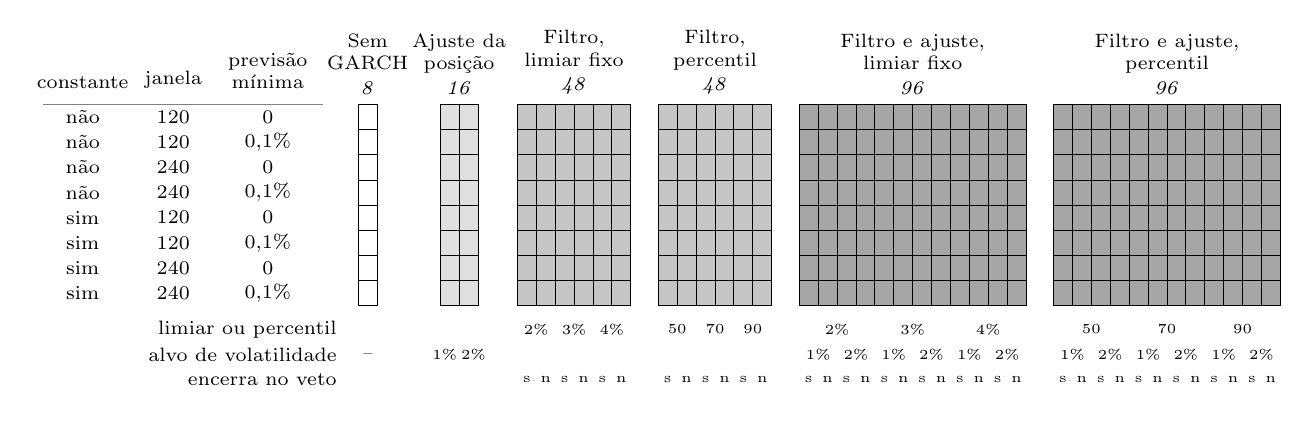
\begin{tikzpicture}
  % combinações comuns a todas as formas (as 8 linhas)
  \node[font=\scriptsize, anchor=south, align=center] at (-3.5, 0.08) {constante};
  \node[font=\scriptsize, anchor=south, align=center] at (-2.35, 0.08) {janela};
  \node[font=\scriptsize, anchor=south, align=center] at (-1.15, 0.08) {previsão\\mínima};
  \foreach \r/\a/\b/\pm in {0/não/120/0, 1/não/120/{0,1\%}, 2/não/240/0, 3/não/240/{0,1\%},
                           4/sim/120/0, 5/sim/120/{0,1\%}, 6/sim/240/0, 7/sim/240/{0,1\%}} {
    \node[font=\scriptsize] at (-3.5, {-\r*\h-\h/2}) {\a};
    \node[font=\scriptsize] at (-2.35, {-\r*\h-\h/2}) {\b};
    \node[font=\scriptsize] at (-1.15, {-\r*\h-\h/2}) {\pm};}
  \draw[gray] (-4.0, 0) -- (-0.45, 0);

  % os seis blocos, um por forma de uso do GARCH
  \bloco{0}{1}{white}            \nome{0}{1}{Sem\\GARCH}{8}
  \bloco{1.04}{2}{gray!25}       \nome{1.04}{2}{Ajuste da\\posição}{16}
  \bloco{2.02}{6}{gray!45}       \nome{2.02}{6}{Filtro,\\limiar fixo}{48}
  \bloco{3.81}{6}{gray!45}       \nome{3.81}{6}{Filtro,\\percentil}{48}
  \bloco{5.60}{12}{gray!70}      \nome{5.60}{12}{Filtro e ajuste,\\limiar fixo}{96}
  \bloco{8.83}{12}{gray!70}      \nome{8.83}{12}{Filtro e ajuste,\\percentil}{96}

  % parâmetros próprios de cada coluna
  \def\yA{-2.86} \def\yB{-3.18} \def\yC{-3.50}
  \node[font=\scriptsize, anchor=east] at (-0.15, \yA) {limiar ou percentil};
  \node[font=\scriptsize, anchor=east] at (-0.15, \yB) {alvo de volatilidade};
  \node[font=\scriptsize, anchor=east] at (-0.15, \yC) {encerra no veto};
  \rotulo{0}{1}{1}{\yB}{--}
  \node[font=\tiny, inner sep=0pt, anchor=east] at ({1.04+\w-0.02}, \yB) {1\%};
  \node[font=\tiny, inner sep=0pt, anchor=west] at ({1.04+\w+0.02}, \yB) {2\%};
  \foreach \x/\v in {2.02/{2\%,3\%,4\%}, 3.81/{50,70,90}} {
    \foreach \t [count=\i] in \v \rotulo{\x}{2*\i-1}{2}{\yA}{\t};
    \foreach \i in {1,3,5} {\rotulo{\x}{\i}{1}{\yC}{s} \rotulo{\x}{\i+1}{1}{\yC}{n}}}
  \foreach \x/\v in {5.60/{2\%,3\%,4\%}, 8.83/{50,70,90}} {
    \foreach \t [count=\i] in \v \rotulo{\x}{4*\i-3}{4}{\yA}{\t};
    \foreach \i in {1,5,9} {\rotulo{\x}{\i}{2}{\yB}{1\%} \rotulo{\x}{\i+2}{2}{\yB}{2\%}}
    \foreach \i in {1,3,...,11} {\rotulo{\x}{\i}{1}{\yC}{s} \rotulo{\x}{\i+1}{1}{\yC}{n}}}
\end{tikzpicture}
\end{document}
